\chapter{Bipolære steppermotorer}

\section{Indledning}
Da der enkelte steder i WinePrep er behov for en større motorkraft end de unipolære stepper motorer kan leveres anvendes der her bipolære stepper motorer
i stedet Dette giver en lidt mere kompleks styring, men en noget større trækkraft.

\section{Teori}
En stepper motor er en elektromotor der kan bevæges i små trin af en bestemt vinkel, ofte 1.8 eller 0.9 grader afhængig af motoren, dette giver en meget
præcis positionering til forskel fra de mere gængse DC motorer der er bedre egnet til kontinuerte bevægelser der skal foregå flydende.

Steppermotorerne har flere fordele, i sammenhæng med WinePrep er de valgt da præcis positionering samt evnen til at gentage denne positionering er vigtig.
Derudover har vi behov for en rigtig god evne til at bevare en given stillestående position på trods af ekstra belastninger, og her kommer stepper motorens
rigtig gode hold torque til sin ret.

Stepper motorer kommer i flere varianter, og i WinePrep anvendes der både bipolare samt unipolare stepper motore. I dette dokument fokuseres der udelukkende
på Bipolare stepper motore. Ønskes der information om brugen af unipolare stepper motore kan denne findes i dokumentet "Unipolære steppermotorer".

\subsection{Bipolar Stepper Motor}

Den bipolære steppermotor adskiller sig som det ses på figur \ref{bipolarlayout} fra den unipolære stepper motor ved at have 1 vikling per fase hvor den
unipolære har 1 fælles tab i midten af spolen.

Afhængig af polariteten i den givne spole vil motoren rotere sin akse til den givne position.

\begin{figure}[H]
	\centering
	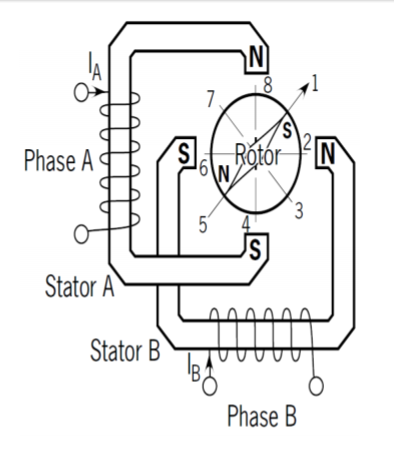
\includegraphics{Billeder/konstruktion}
	\caption{Biporlar stepper motors konstruktion}
	\label{bipolarlayout}
\end{figure}

Til WinePrep anvedes der kun stepper motorer med gearing, hvilket gør at vi ikke anvender microstepping, da vi allerede uden dette har en rigelig god præcision.

For at anvende en bipolar stepper til full step skal faserne påtrykkes spænding ud fra lookup tabellen på figur \ref{lookuptabel}.

\begin{figure}[H]
	\centering
	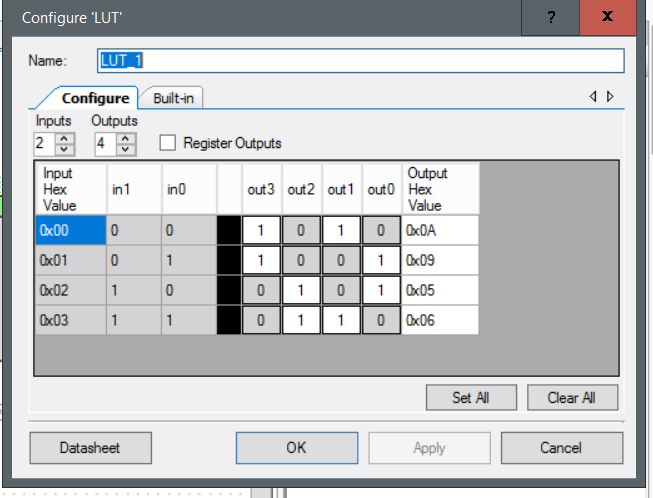
\includegraphics{Billeder/lookup}
	\caption{lookup tabel for bipolar stepper motor}
	\label{lookuptabel}
\end{figure}

Den bipolare stepper motor styres med 1 fuld h-bro pr fase.

\section{Design}
Til at styre de Bipolære stepper motorer anvendes der et print designet omkring chippen L298, der er en dual full-bridge driver.

På blok diagrammet for L298 der kan ses på figur \ref{blok298}, ses det at chippen indeholde mulighed for at lave et strøm feedback loop tilbage til PSoC 5
Chippen hvor man ved hjælp af en comparator og en DAC kan sikre sig mod for store strømme i stepper motoren. 

Derudover kan man se hvordan brugen af AND-Gates kan medføre en besparelse i antallet af pins der er nødvendige for at drive en full-bridge.

\begin{figure}[H]
	\centering
	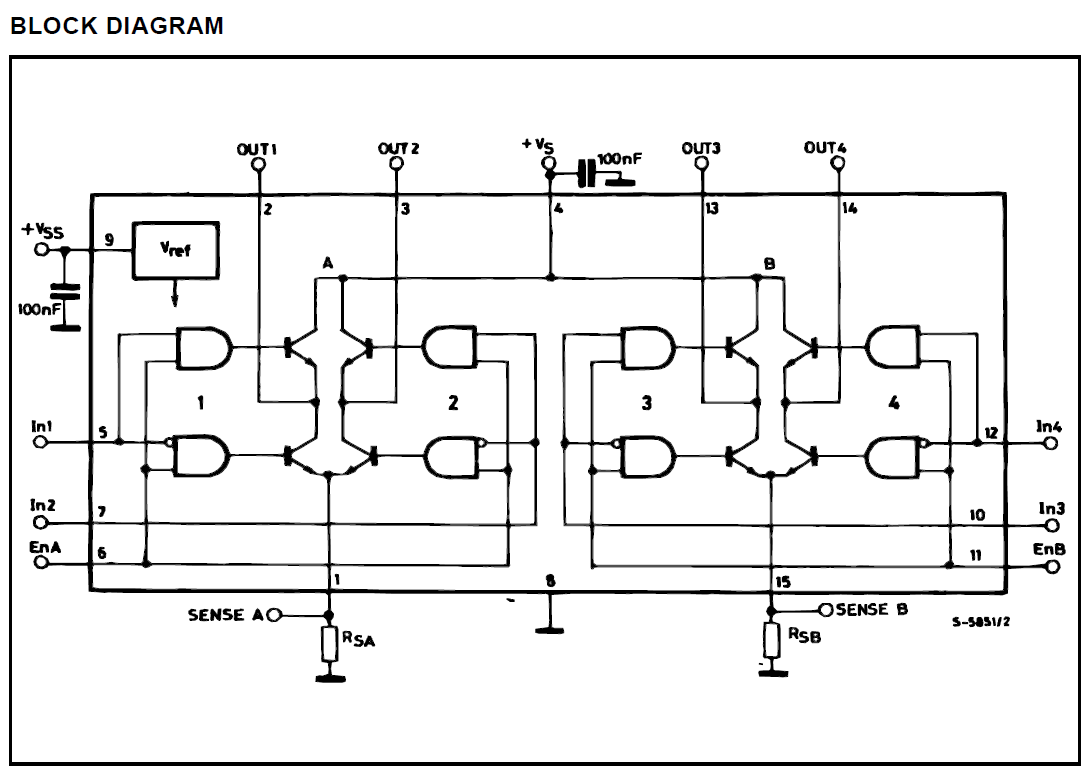
\includegraphics[scale=0.5]{Billeder/blokdiagramL298}
	\caption{Blokdiagram for L298, kilde: datablad for L298}
	\label{blok298}
\end{figure}

Denne forsynes via 12V og 78L05 DC-DC 5V konverteren på boardet med 5V til de logiske enheder på chippen.

Derudover er der som anbefalet i databladet for 78L05 sat kondensatorer til at stabiliserer 5V forsyningen, samt på L298 ud fra anbefalinger i databladet.

\begin{figure}[H]
	\centering
	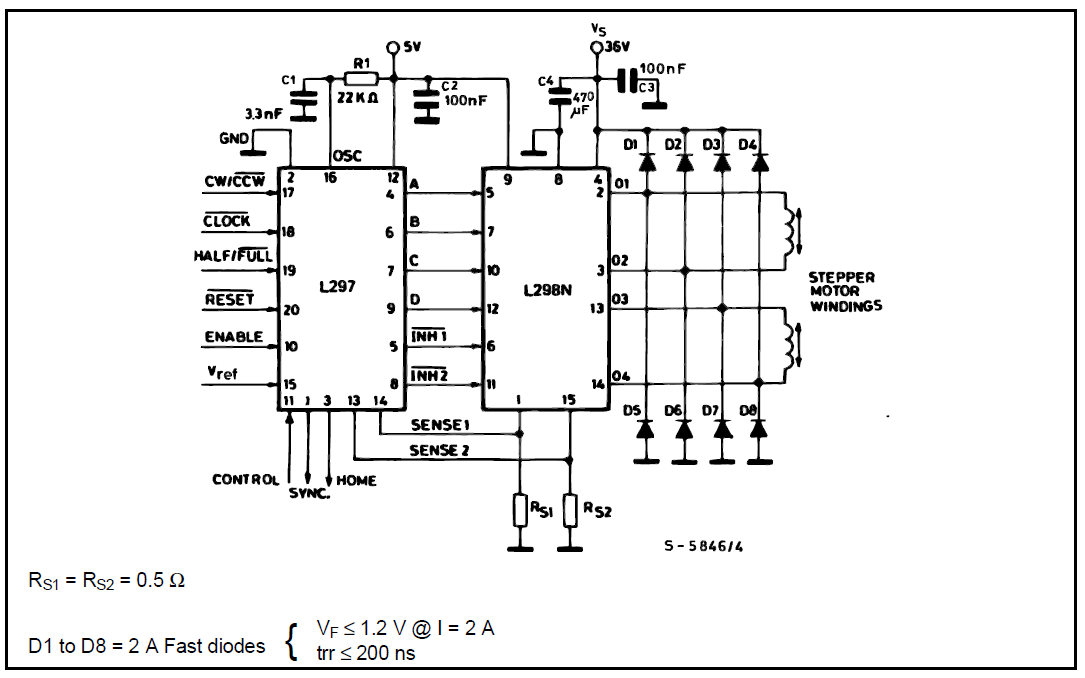
\includegraphics[scale=0.5]{Billeder/kredsloebL297L298}
	\caption{kredsløb til styring a bipolar steppermotor med L298 samt L297. Kilde: datablad L298.}
	\label{L298L297}
\end{figure}

Der er i designfasen taget udgangspunkt i kredsløbet der ses på Figur \ref{L298L297} , i vores kredsløb er L297 dog erstattet af en PSoC5LP og der er anvendt
andre modstande til strømsfeedback delen, da vi ikke havde den samme type på lager på skolen.

Der i som RS1 og RS2 istedet anvendt en 0.1 ohm effektmodstand, da de små 1/4 watts modstande ikke ville kunne tåle de strømme der vil kunne løbe igennem motoren.

Dette giver os ud fra kirchoffs strømlov at strømmen gennem RS1 er den samme som strømmen gennem spolen på stepper motoren, derved kan vi ved hjælp af ohms lov
finde frem til den spænding vi skal indstille vores DAC i PSoC5LP til, for at vi opnår den ønskede strøm i motoren.

Den generelle formel findes i ligning \ref{Currentfeedback-general} hvorfra en mere specifik udgave der kun vil passe på vores kredsløb kan findes på i ligning
\ref{Currentfeedback-specific}

\begin{equation}
\label{Currentfeedback-general}
	\frac{I_{spole}}{R_{S1}}=V_{DAC}
\end{equation}

\begin{equation}
\label{Currentfeedback-specific}
\frac{I_{spole}}{0.1\Omega}=V_{DAC}
\end{equation}

\section{Implementering}
Ud fra dette og de tilgængelige komponenter på vores komponentalger er vi kommet frem til et print design der ser ud som på figur \ref{printdesign}.

\begin{figure}[H]
	\centering
	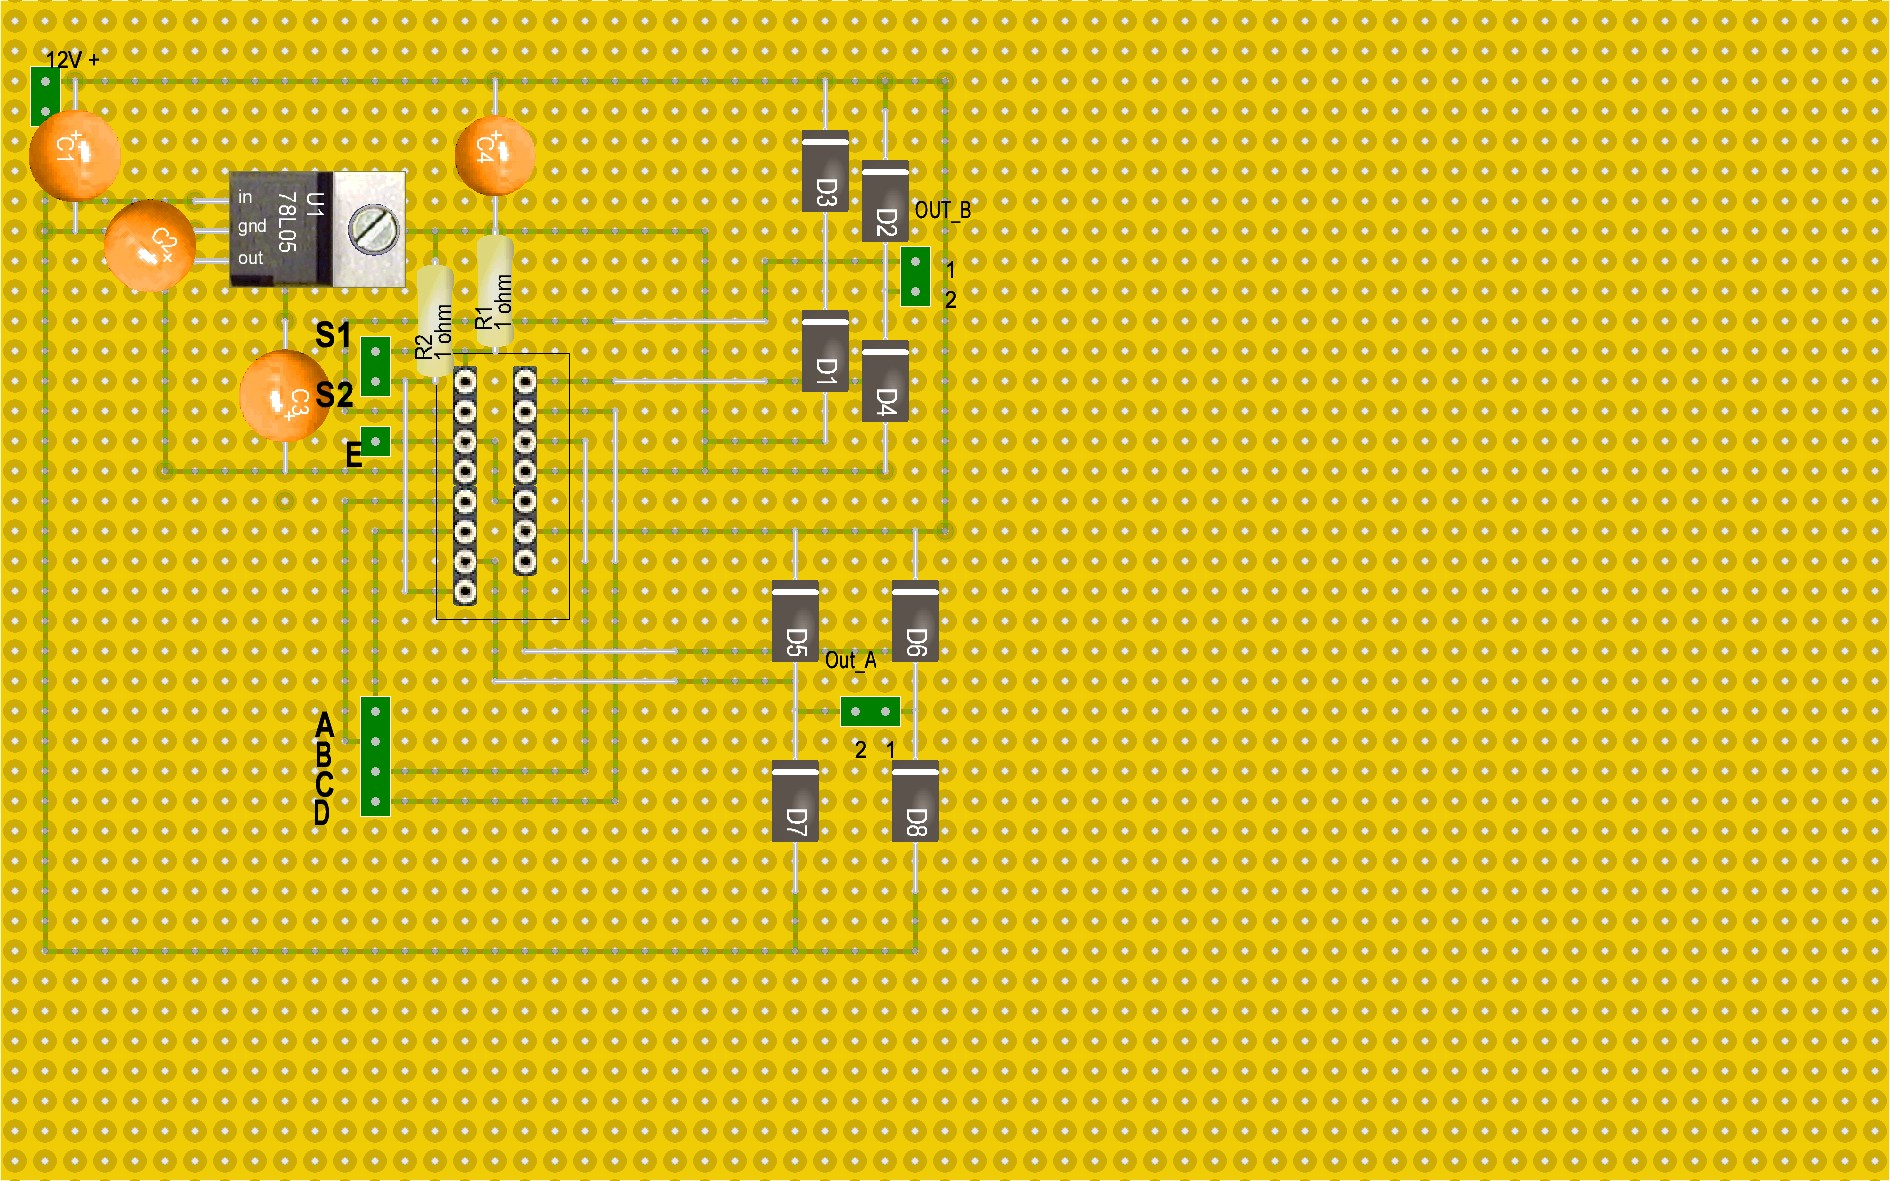
\includegraphics[scale=0.25,trim=0 20 500 0, clip]{Billeder/printdesign}
	\caption{Resulterende printdesign}
	\label{printdesign}
\end{figure}

De anvendte dioder er af typen 1N4148 og anvendes som flybackdioder for at beskytte L298 mod de strømme der opstår når spolerne slukkes.

Kondensatorene på det endelig print er ikke af tantalum typen, men værdier er de foreskrevne i databladet for L298.

Det færdige print ses på Figur \ref{solderedprint}.

\begin{figure}[H]
	\centering
	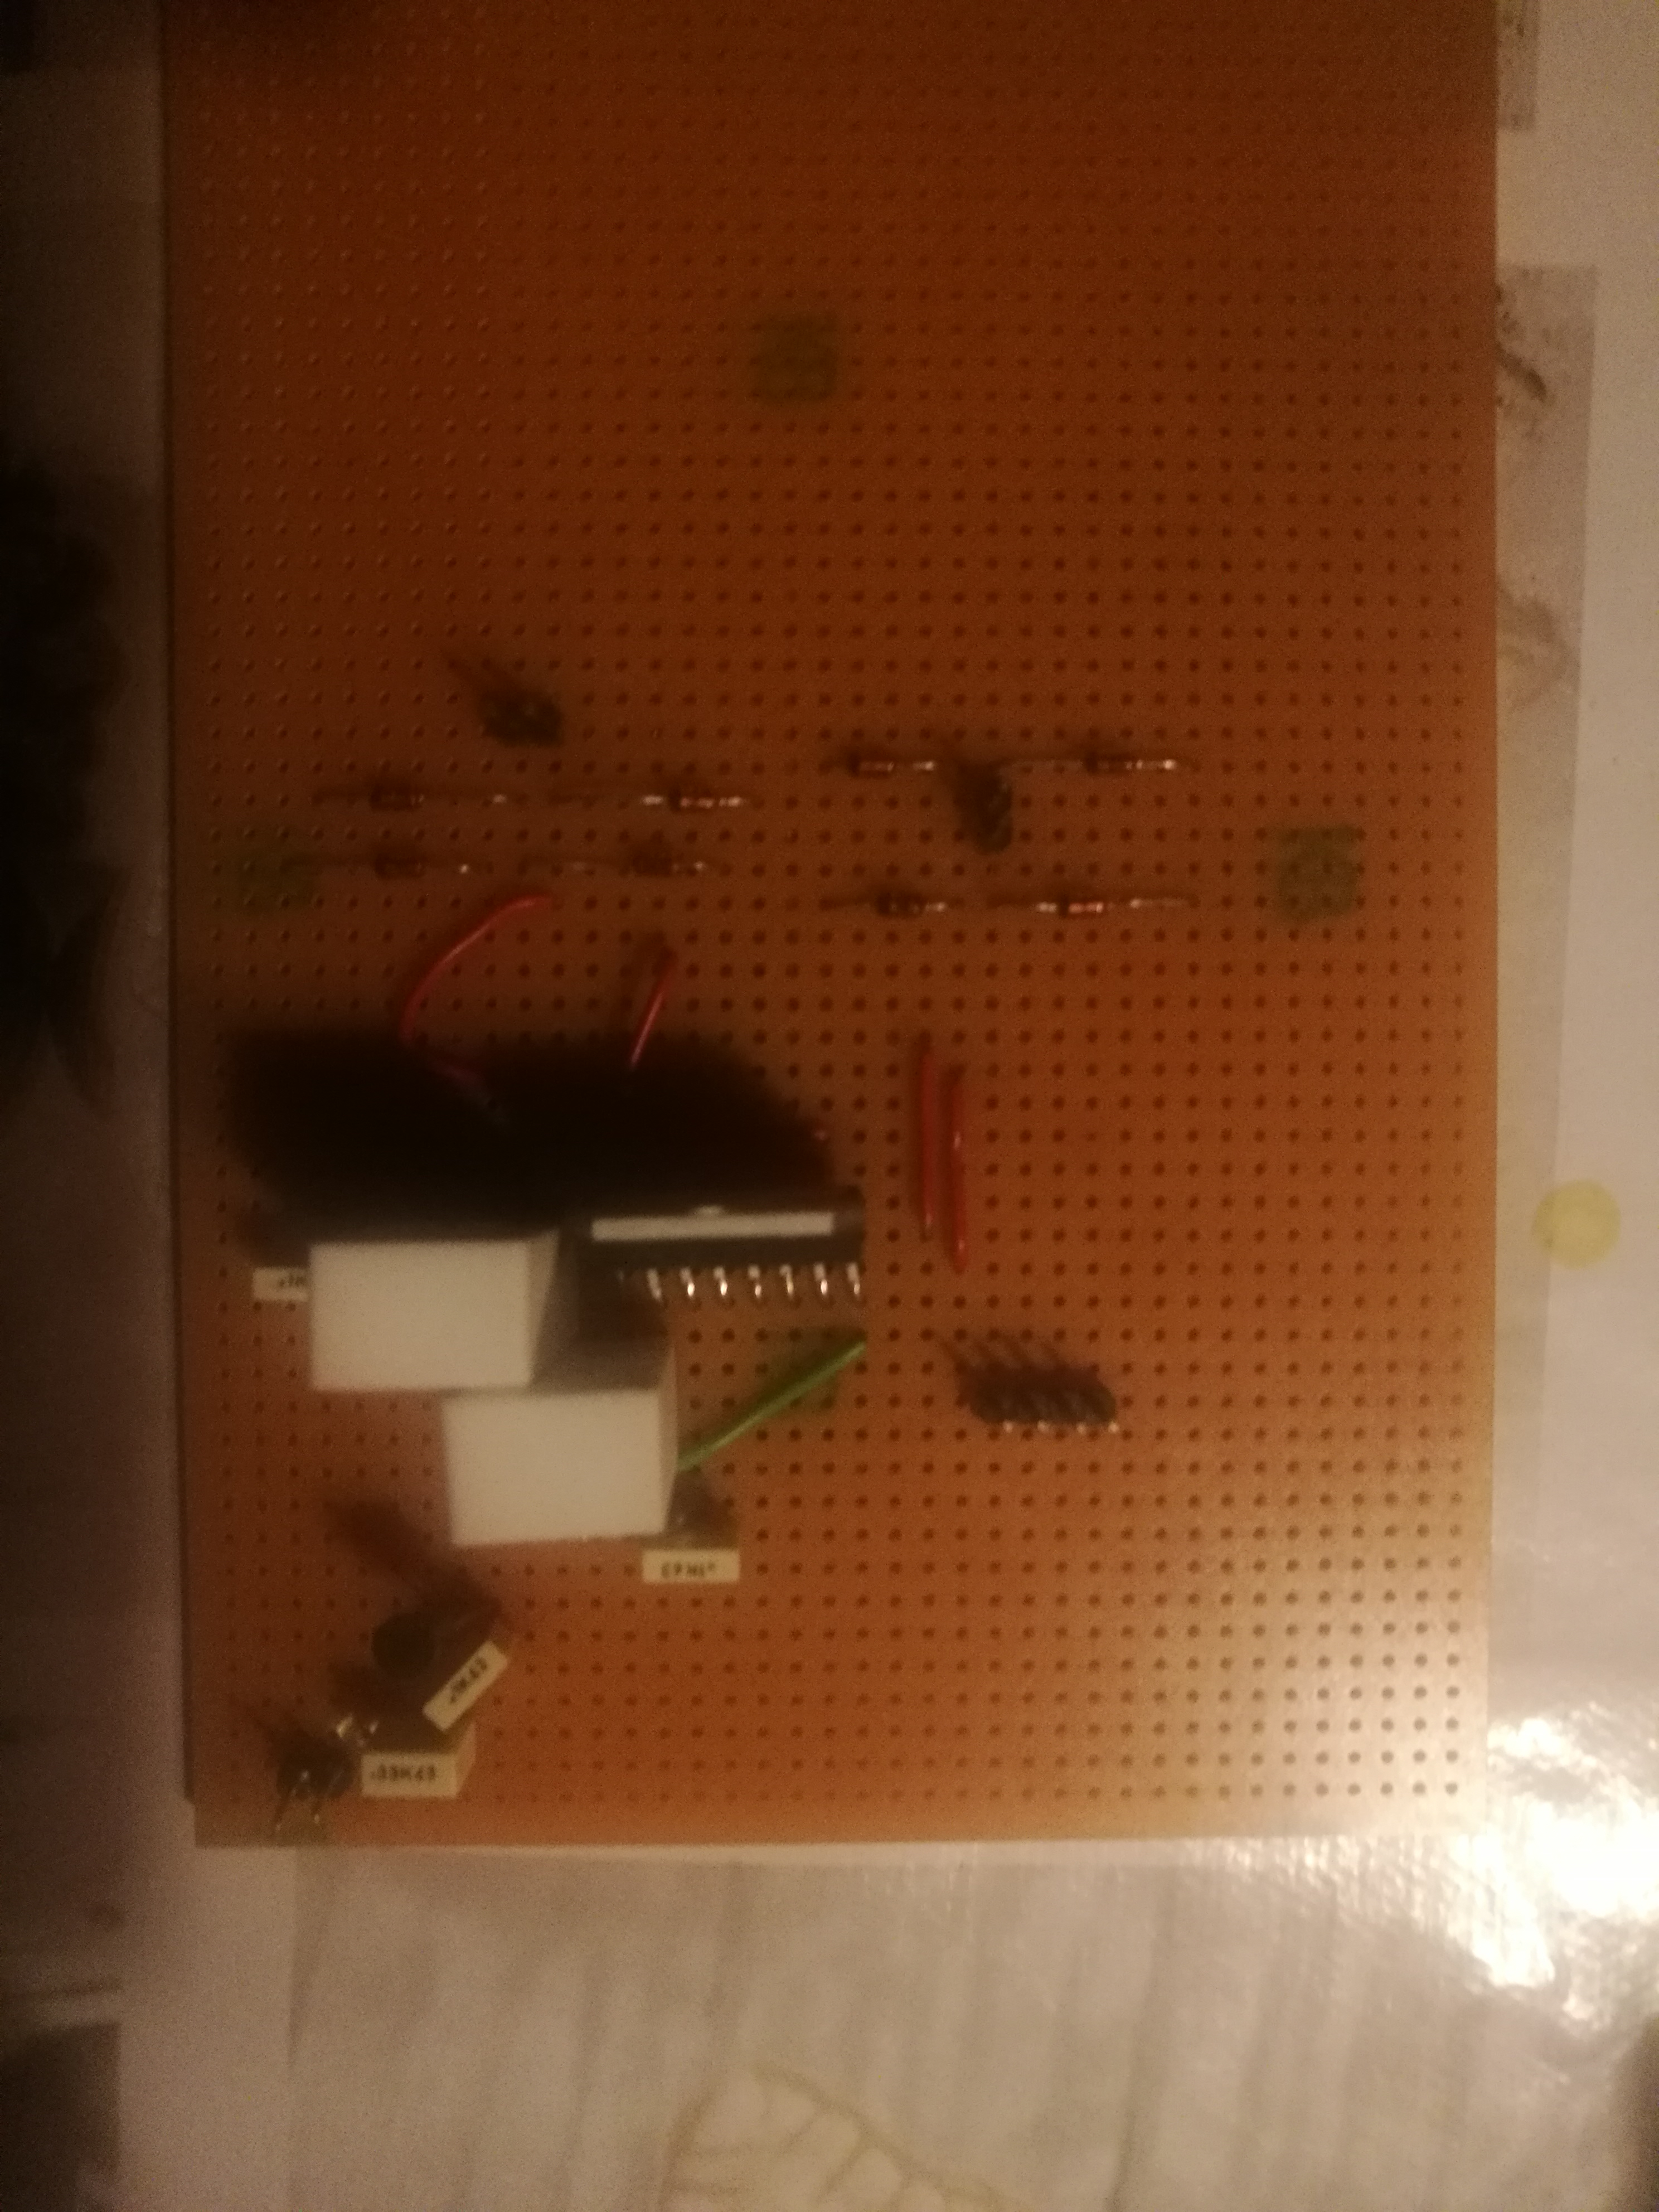
\includegraphics[scale=0.1,trim=0 0 0 0, clip]{Billeder/solderedprint.jpg}
	\caption{Resulterende print}
	\label{solderedprint}
\end{figure}

\section{Test og resultater}
Test resultater mangler da software til styringen ikke er fuldt funktionel endnu.

Problemet med softwaren på nuværende tidspunkt at at PWM delen i PSoC generere et 14 kHz 50\% dutycycle puls signal hvor den burde være lav.

\section{Konklusion}
Mangler grundet manglende test.
